% Created 2014-04-26 Sat 00:04
\documentclass[table,smaller]{beamer}
\usepackage[utf8]{inputenc}
\usepackage[T1]{fontenc}
\usepackage{fixltx2e}
\usepackage{graphicx}
\usepackage{longtable}
\usepackage{float}
\usepackage{wrapfig}
\usepackage{rotating}
\usepackage[normalem]{ulem}
\usepackage{amsmath}
\usepackage{textcomp}
\usepackage{marvosym}
\usepackage{wasysym}
\usepackage{amssymb}
\usepackage{hyperref}
\tolerance=1000
\usepackage{tikz}
\usepackage{minted}
\usepackage{fancyvrb}
\usemintedstyle{perldoc}
\definecolor{lightgray}{gray}{0.96}
\setlength{\tabcolsep}{1ex}
\usetheme{Warsaw}
\useoutertheme{infolines}
\setbeamercolor{block body}{bg=lightgray}
\titlegraphic{
\includegraphics[width=.75\textwidth]{images/IQSSNewLogo.pdf}}
\setbeamersize{text margin left=2em,text margin right=2em}
\AtBeginSection[]{\begin{frame}<beamer>\frametitle{Topic}\tableofcontents[currentsection]\end{frame}}
\usetheme{default}
\author{}
\date{}
\title{Introduciton to R Graphics with \texttt{ggplot2}}
\hypersetup{
  pdfkeywords={},
  pdfsubject={},
  pdfcreator={Emacs 24.3.1 (Org mode 8.2.5h)}}
\begin{document}

\maketitle
\begin{frame}{Outline}
\tableofcontents
\end{frame}



\section{Introduction}
\label{sec-1}

\begin{frame}[fragile,label=sec-1-1]{Class Files And Administrative Details}
 \begin{itemize}
\item User name: dataclass
\item Password: dataclass
\item Copy \alert{Rgraphics} folder from shared drive to your desktop
\item Class Structure and Organization
\begin{itemize}
\item Ask questions at any time. Really!
\item Collaboration is encouraged
\item This is your class! Special requests are encouraged
\end{itemize}
\item This is an intermediate R course
\begin{itemize}
\item Assumes working knowledge of R
\item Relatively fast-paced
\item Focus is on \texttt{ggplot2} graphics--other packages will not be covered
\end{itemize}
\end{itemize}
\end{frame}

\begin{frame}[label=sec-1-2]{Starting A The End}
My goal: by the end of the workshop you will be able to reproduce this graphic from the Economist:

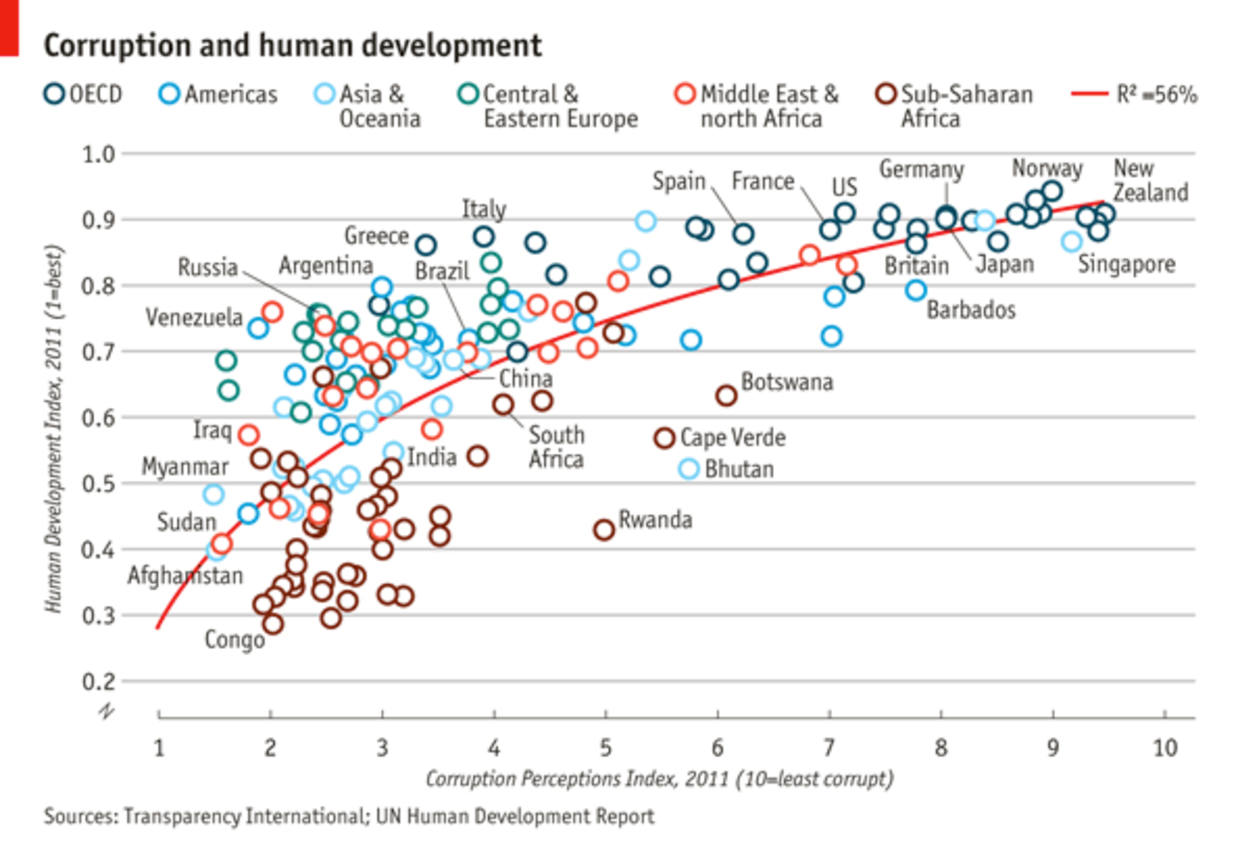
\includegraphics[width=.9\linewidth]{images/Economist1.pdf}
\end{frame}


\begin{frame}[fragile,label=sec-1-3]{Why \texttt{ggplot2}?}
 \begin{itemize}
\item Advantages of ggplot2
\begin{itemize}
\item Consistent underlying \texttt{grammar of graphics} (Wilkinson, 2005)
\item Plot specification at a high level of abstraction
\item Very flexible
\item Theme system for polishing plot appearance
\item Active maintenance and development--getting better all the time
\item Many users, active mailing list
\end{itemize}
\item Things you cannot do With ggplot2
\begin{itemize}
\item 3-dimensional graphics
\item Graph-theory type graphs (nodes/edges layout)
\end{itemize}
\end{itemize}
\end{frame}

\begin{frame}[label=sec-1-4]{What Is The Grammar Of Graphics?}
\begin{itemize}
\item The basic idea: independently specify plot building blocks
\item Anatomy of a plot:
\begin{itemize}
\item data
\item aesthetic mapping
\item geometric object
\item statistical transformations
\item scales
\item coordinate system
\item position adjustments
\item faceting
\end{itemize}
\end{itemize}
\end{frame}

\begin{frame}[fragile,label=sec-1-5]{The structure of a \texttt{ggplot}}
 The  \texttt{ggplot()} function is used to initialize the basic graph structure, then we add to it. The structure of a ggplot looks like this:
\begin{columns} \column{.85\textwidth}
\begin{minted}[fontsize=\scriptsize]{r}
ggplot(data = <default data set>, 
       aes(x = <default x axis variable>,
	   y = <default y axis variable>,
	   ... <other default aesthetic mappings>),
       ... <other plot defaults>) +
       geom_<geom type>(aes(size = <size variable for this geom>, 
		      ... <other aesthetic mappings>),
		  data = <data for this point geom>,
		  stat = <statistic string or function>,
		  position = <position string or function>,
		  color = <"fixed color specification">,
		  <other arguments, possibly passed to the _stat_ function) +
  scale_<aesthetic>_<type>(name = <"scale label">,
		     breaks = <where to put tick marks>,
		     labels = <labels for tick marks>,
		     ... <other options for the scale>) +
  theme(plot.background = element_rect(fill = "gray"),
	... <other theme elements>)
\end{minted}
\vspace{-2em}
\end{columns}
\begin{itemize}
\item Don't be afraid, you will understand this by the end of the workshop!
\item The basic idea is that you specify different parts of the plot, and add them together using the "+" operator
\end{itemize}
\end{frame}

\begin{frame}[fragile,label=sec-1-6]{Example data I: \texttt{mtcars}}
 \tiny

\begin{minted}[fontsize=\scriptsize]{r}
print(head(mtcars, 4))
\end{minted}
\vspace{-2em}

\vspace{-.5em}
\begin{columns}
\column{.95\linewidth}
\begin{block}{}
\begin{minted}[linenos=false, fontsize=\footnotesize]{rconsole}
mpg	Miles/(US) gallon			 
cyl	Number of cylinders			 
disp	Displacement (cu.in.)			 
hp	Gross horsepower			 
drat	Rear axle ratio				 
wt	Weight (lb/1000)			 
qsec	1/4 mile time				 
vs	V/S					 
am	Transmission (0 = automatic, 1 = manual) 
gear	Number of forward gears			 
carb	Number of carburetors
\end{minted}
\end{block}
\end{columns}
\vspace{.5em}

\normalsize
\end{frame}

\begin{frame}[fragile,label=sec-1-7]{\texttt{ggplot2} VS Base Graphics}
 \begin{itemize}
\item Compared to base graphics, \texttt{ggplot2}
\begin{itemize}
\item is more verbose for simple / canned graphics
\item is less verbose for complex / custom graphics
\item does not have methods (data should always be in a \texttt{data.frame})
\item uses a different system for adding plot elements
\end{itemize}
\end{itemize}
\end{frame}

\begin{frame}[fragile,label=sec-1-8]{\texttt{ggplot2} VS Base Graphics}
 Base graphics VS \texttt{ggplot} for simple graphs:
\begin{columns}
\begin{column}{0.5\textwidth}

\begin{columns} \column{.85\textwidth} \begin{block}{}

\begin{minted}[fontsize=\scriptsize]{r}
hist(mtcars$mpg)
\end{minted}

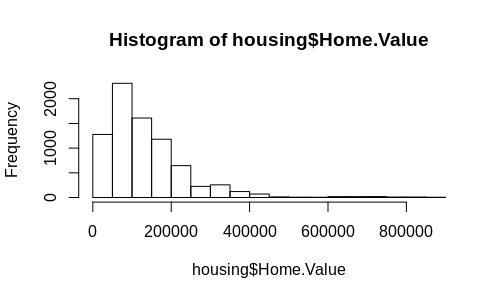
\includegraphics[width=.9\linewidth]{images/baseHist1.png}
\end{block} \end{columns}
\end{column}
\begin{column}{0.5\textwidth}

\begin{columns} \column{.85\textwidth} \begin{block}{}

\begin{minted}[fontsize=\scriptsize]{r}
ggplot(mtcars, aes(x = mpg)) +
  geom_histogram(binwidth = 5)
\end{minted}

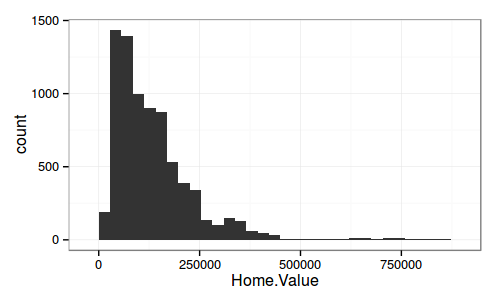
\includegraphics[width=.9\linewidth]{images/ggplotHist1.png}
\end{block} \end{columns}
\end{column}

\begin{column}{1.0\textwidth}

\end{column}
\end{columns}
\end{frame}

\begin{frame}[fragile,label=sec-1-9]{\texttt{ggplot2} VS Base Graphics}
 Base graphics VS \texttt{ggplot} for complex graphs:
\begin{columns}
\begin{column}{0.5\textwidth}

\begin{columns} \column{.85\textwidth} \begin{block}{}

\begin{minted}[fontsize=\scriptsize]{r}
par(mar = c(4,4,.1,.1))
plot(mpg ~ hp,
     data=subset(mtcars, am==1),
     xlim=c(50, 450),ylim=c(5, 40))
points(mpg ~ hp, col="red",
       data=subset(mtcars, am==0))
legend(350, 40,
       c("1", "0"), title="am",
       col=c("black", "red"),
       pch=c(1, 1))
\end{minted}

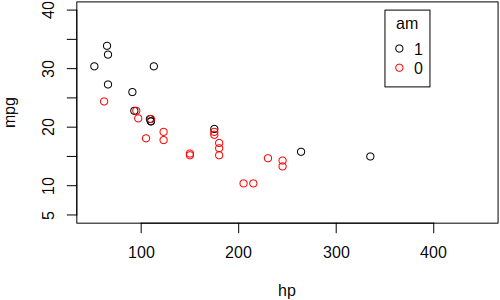
\includegraphics[width=.9\linewidth]{images/baseComplex1.png}

\end{block} \end{columns}
\end{column}
\begin{column}{0.5\textwidth}

\begin{columns} \column{.85\textwidth} \begin{block}{}

\begin{minted}[fontsize=\scriptsize]{r}
ggplot(mtcars, aes(x=hp,
	      y=mpg,
	      color=factor(am)))+
geom_point()




#
\end{minted}

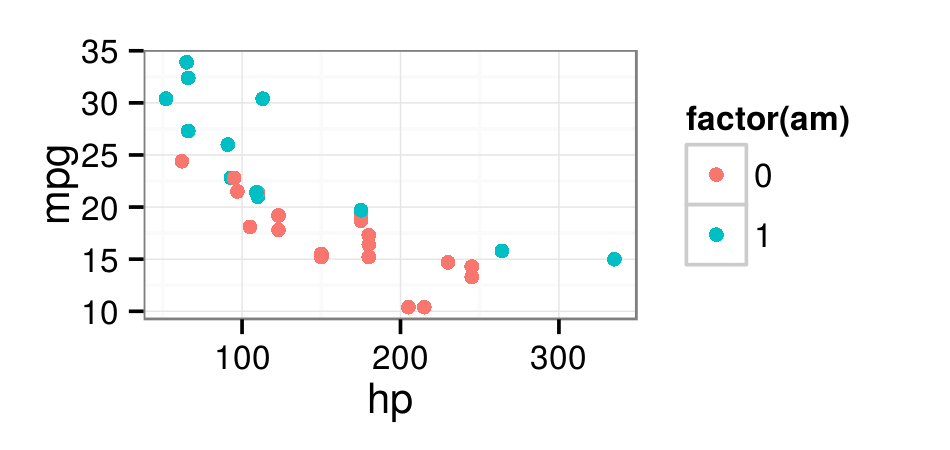
\includegraphics[width=.9\linewidth]{images/ggplotComplex1.png}

\end{block} \end{columns}
\end{column}


\begin{column}{1.0\textwidth}

\end{column}
\end{columns}
\end{frame}

\section{Geometric Objects And Aesthetics}
\label{sec-2}

\begin{frame}[fragile,label=sec-2-1]{Aesthetic Mapping}
 \begin{itemize}
\item In ggplot land \emph{aesthetic} means "something you can see"
\item Examples include:
\begin{itemize}
\item position (i.e., on the x and y axes)
\item color ("outside" color)
\item fill ("inside" color)
\item shape (of points)
\item linetype
\item size
\end{itemize}
\item Each type of geom accepts only a subset of all aesthetics--refer to the geom help pages to see what mappings each geom accepts
\item Aesthetic mappings are set with the \texttt{aes()} function
\end{itemize}
\end{frame}

\begin{frame}[fragile,label=sec-2-2]{Geometic Objects (\texttt{geom})}
 \begin{itemize}
\item Geometric objects are the actual marks we put on a plot
\item Examples include:
\begin{itemize}
\item points (\texttt{geom\_point}, for scatter plots, dot plots, etc)
\item lines (\texttt{geom\_line}, for time series, trend lines, etc)
\item boxplot (\texttt{geom\_boxplot}, for, well, boxplots!)
\end{itemize}
\item A plot must have at least one geom; there is no upper limit
\item Add a geom to a plot using the \texttt{+} operator
\item You can get a list of available geometric objects:
\end{itemize}
\begin{minted}[fontsize=\scriptsize]{r}
geoms <- help.search("geom_", package = "ggplot2")
geoms$matches[1:4, 1:2]
\end{minted}
\end{frame}

\begin{frame}[fragile,label=sec-2-3]{Points (Scatterplot)}
 \begin{itemize}
\item Now that we know about geometric objects and aesthetic mapping, we can make a ggplot
\end{itemize}
\begin{columns}
\begin{column}{0.5\textwidth}

\begin{columns} \column{.85\textwidth} \begin{block}{}

\begin{minted}[fontsize=\scriptsize]{r}
ggplot(mtcars, aes(x = hp, y = mpg)) +
  geom_point()
\end{minted}

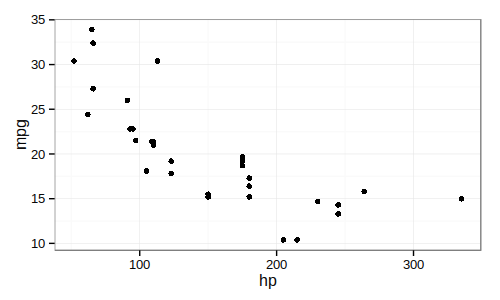
\includegraphics[width=.9\linewidth]{images/firstScatter.png}
\end{block} \end{columns}
\end{column}

\begin{column}{0.5\textwidth}

\begin{columns} \column{.85\textwidth} \begin{block}{}

\begin{minted}[fontsize=\scriptsize]{r}
ggplot(mtcars, aes(x = hp, y = mpg)) +
  geom_point(aes(y=log10(mpg)))
\end{minted}

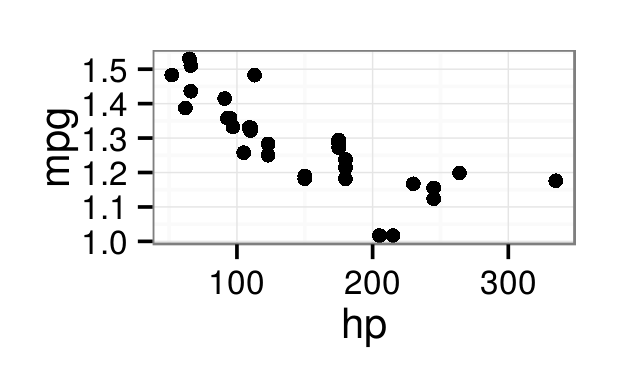
\includegraphics[width=.9\linewidth]{images/overrideScatterDefault.png}
\end{block} \end{columns}
\end{column}
\end{columns}
\end{frame}

\begin{frame}[fragile,label=sec-2-4]{Lines (Prediction Line)}
 \begin{itemize}
\item A plot constructed with \texttt{ggplot} can have more than one geom

\item Our \texttt{hp} vs \texttt{mpg} plot could use a regression line:
\end{itemize}

\begin{columns} \column{.85\textwidth} \begin{block}{}

\begin{minted}[fontsize=\scriptsize]{r}
mtcars$pred.mpg <- predict(lm(mpg ~ hp, data = mtcars))

p1 <- ggplot(mtcars, aes(x = hp, y = mpg))

p1 + geom_point(aes(color = wt)) +
  geom_line(aes(y = pred.mpg))
\end{minted}

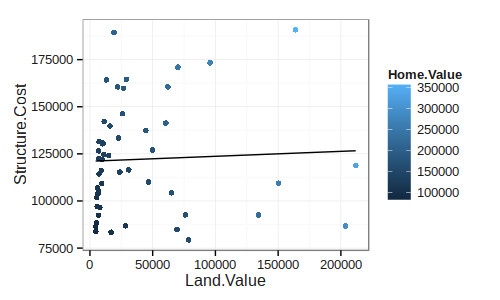
\includegraphics[width=.9\linewidth]{images/mtcarsLayers.png}

\end{block} \end{columns}
\end{frame}

\begin{frame}[fragile,label=sec-2-5]{Smoothers}
 \begin{itemize}
\item Not all geometric objects are simple shapes--the smooth geom includes a line and a ribbon
\end{itemize}

\begin{columns} \column{.85\textwidth} \begin{block}{}

\begin{minted}[fontsize=\scriptsize]{r}
p2 <- ggplot(mtcars, aes(x = hp, y = mpg))

p2 + geom_point(aes(color = wt)) +
  geom_smooth()
\end{minted}

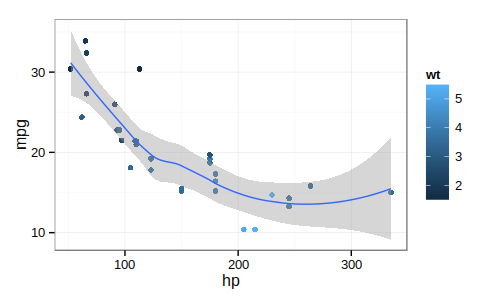
\includegraphics[width=.9\linewidth]{images/mtcarsLayers2.png}
\end{block} \end{columns}
\end{frame}

\begin{frame}[fragile,label=sec-2-6]{Text (Label Points)}
 \begin{itemize}
\item Each \texttt{geom} accepts a particualar set of mappings--for example \texttt{geom\_text()} accepts a \texttt{labels} mapping
\end{itemize}

\begin{columns} \column{.85\textwidth} \begin{block}{}

\begin{minted}[fontsize=\scriptsize]{r}
p2 + geom_point(aes(color = wt)) +
  geom_smooth() +
  geom_text(aes(label=rownames(mtcars)), size=2)
\end{minted}

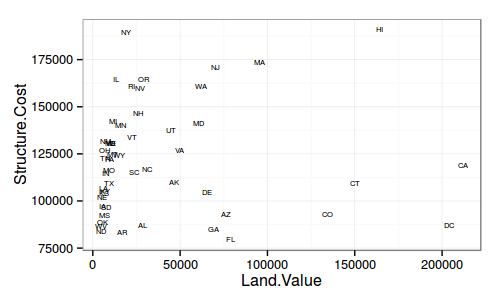
\includegraphics[width=.9\linewidth]{images/textGeomMapping.png}

\end{block} \end{columns}
\end{frame}

\begin{frame}[fragile,label=sec-2-7]{Aesthetic Mapping VS Assignment}
 \begin{itemize}
\item Note that variables are mapped to aesthetics with the \texttt{aes()} function, while fixed aesthetics are set outside the aes() call
\item This sometimes leads to confusion, as in this example:
\end{itemize}

\begin{columns} \column{.85\textwidth} \begin{block}{}

\begin{minted}[fontsize=\scriptsize]{r}
ggplot(mtcars, aes(x = hp, y = mpg)) +
  geom_point(aes(size = 2),# incorrect! 2 is not a variable
	     color="red") # this is fine -- all points red
\end{minted}

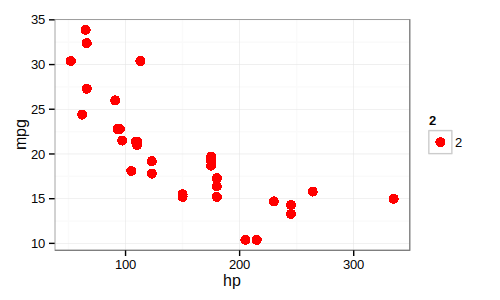
\includegraphics[width=.9\linewidth]{images/mtcars2.png}

\end{block} \end{columns}
\end{frame}

\begin{frame}[fragile,label=sec-2-8]{Mapping Variables To Other Aesthetics}
 \begin{itemize}
\item Other aesthetics are mapped in the same way as x and y in the previous example
\end{itemize}

\begin{columns} \column{.85\textwidth} \begin{block}{}

\begin{minted}[fontsize=\scriptsize]{r}
ggplot(mtcars, aes(x = hp, y = mpg)) +
  geom_point(aes(color=wt, shape = factor(am)))
\end{minted}

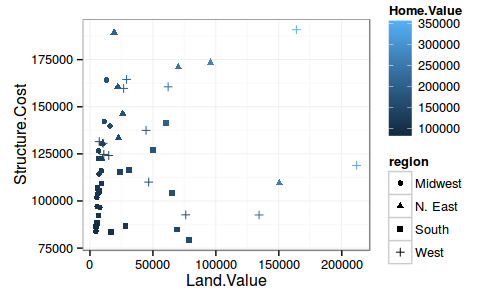
\includegraphics[width=.9\linewidth]{images/addColorAndShapeMapping.png}

\end{block} \end{columns}
\end{frame}

\begin{frame}[fragile,label=sec-2-9]{Exercise I}
 \begin{enumerate}
\item Create a scatter plot with displacement on the \texttt{x} axis and horse power on the y axis
\item Color the points in the previous plot blue
\item Color the points in the previous plot according to miles per gallon
\end{enumerate}
\end{frame}

\begin{frame}[fragile,label=sec-2-10]{Exercise I prototype}
 \begin{minted}[fontsize=\scriptsize]{r}
					# ex1.1
(p.ex1 <- ggplot(mtcars, aes(x = disp, y = hp)) + geom_point())
					# ex1.2
p.ex1 + geom_point(color = "blue")
					# ex1.3
p.ex1 + geom_point(aes(color = mpg))
\end{minted}
\end{frame}

\section{Statistical Transformations}
\label{sec-3}

\begin{frame}[fragile,label=sec-3-1]{Statistical Transformations}
 \begin{itemize}
\item Some plot types (such as scatterplots) do not require transformations--each point is plotted at x and y coordinates equal to the original value
\item Other plots, such as boxplots, histograms, prediction lines etc. require statistical transformations
\begin{itemize}
\item For a boxplot the y values must be transformed to the median and 1.5(IQR)
\item For a smoother smother the y values must be transformed into predicted values
\end{itemize}
\item Each \texttt{geom} has a default statistic, but these can be changed
\item For example, the default statistic for \texttt{geom\_bar} is \texttt{stat\_bin}
\end{itemize}
\begin{minted}[fontsize=\scriptsize]{r}
args(geom_bar)
# ?stat_bin
\end{minted}
\end{frame}

\begin{frame}[fragile,label=sec-3-2]{Setting Statistical Transformation Arguments}
 \begin{itemize}
\item Arguments to \texttt{stat\_} functions are passed through \texttt{geom\_} functions
\item Slightly annoying because in order to change it you have to first determine which stat the geom uses, then determine the arguments to that stat
\end{itemize}

\begin{columns}
\begin{column}{0.5\textwidth}

\begin{columns} \column{.85\textwidth} \begin{block}{}

\begin{minted}[fontsize=\scriptsize]{r}
ggplot(mtcars, aes(x = mpg)) +
  geom_bar()
\end{minted}

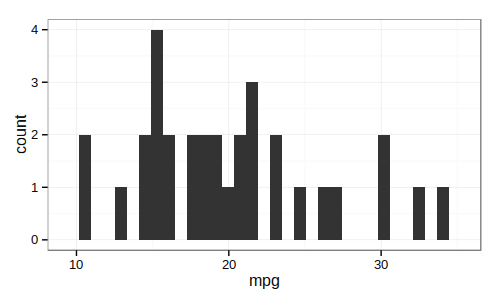
\includegraphics[width=.9\linewidth]{images/GeomBinDefaults.png}

\end{block} \end{columns}
\end{column}

\begin{column}{0.5\textwidth}

\begin{columns} \column{.85\textwidth} \begin{block}{}

\begin{minted}[fontsize=\scriptsize]{r}
ggplot(mtcars, aes(x = mpg)) +
  geom_bar(stat = "bin", binwidth=4)
\end{minted}

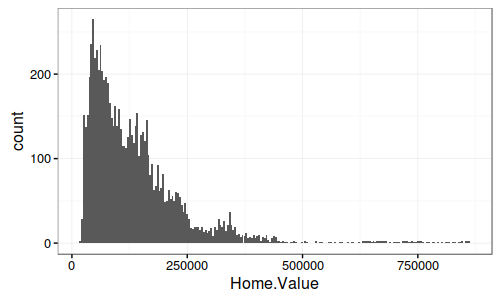
\includegraphics[width=.9\linewidth]{images/ChangeStatBinArgs.png}
\end{block} \end{columns}
\end{column}
\end{columns}
\end{frame}

\begin{frame}[fragile,label=sec-3-3]{Changing The Statistical Transformation}
 \begin{itemize}
\item Sometimes the default statistical transformation is not what you need
\item Often the case with pre-summarized data
\end{itemize}
\begin{minted}[fontsize=\scriptsize]{r}
(mtc.sum <- aggregate(mtcars["mpg"], mtcars["gear"], FUN=mean))
\end{minted}

\begin{columns}
\begin{column}{0.5\textwidth}

\vspace{-.5em}
\begin{columns}
\column{.95\linewidth}
\begin{block}{}
\begin{minted}[linenos=false, fontsize=\footnotesize]{rconsole}
> ggplot(mtc.sum, aes(x=gear, y=mpg)) + 
    geom_bar()
Mapping a variable to y and also 
using stat="bin".
Error in pmin(y, 0) : object 
'y' not found

.
\end{minted}
\end{block}
\end{columns}
\vspace{.5em}
\end{column}

\begin{column}{0.5\textwidth}

\begin{columns} \column{.85\textwidth} \begin{block}{}

\begin{minted}[fontsize=\scriptsize]{r}
ggplot(mtc.sum, aes(x=gear, y=mpg)) + 
  geom_bar(stat="identity")
\end{minted}

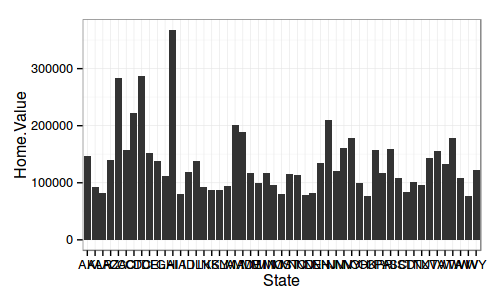
\includegraphics[width=.9\linewidth]{images/ChangeStat.png}

\end{block} \end{columns}
\end{column}
\end{columns}
\end{frame}

\begin{frame}[label=sec-3-4]{Exercise II}
\begin{enumerate}
\item Create boxplots of mpg by gear
\item Overlay points on top of the box plots
\item Create a scatter plot of weight vs. horsepower
\item Overlay a linear regression line on top of the scatter plot
\end{enumerate}
\end{frame}


\begin{frame}[fragile,label=sec-3-5]{Exercise II Prototype}
 \begin{minted}[fontsize=\scriptsize]{r}
					#Ex2.1
(p <- ggplot(mtcars, aes(x = factor(gear), y = mpg)) + geom_boxplot())
					#Ex2.2
p + geom_point()
					#Ex2.3
(p <- ggplot(mtcars, aes(x = wt, y = hp)) + geom_point())
					#Ex2.4
p + geom_smooth(method = "lm")
\end{minted}
\end{frame}


\section{Scales}
\label{sec-4}

\begin{frame}[fragile,label=sec-4-1]{Scales: Controlling Aesthetic Mapping}
 \begin{itemize}
\item In \texttt{ggplot2} \alert{scales} include
\begin{itemize}
\item position
\item color and fill
\item size
\item shape
\item line type
\end{itemize}
\item Modified with \texttt{scale\_<aesthetic>\_<type>}
\end{itemize}
\end{frame}

\begin{frame}[label=sec-4-2]{Common Scale Arguments}
\begin{itemize}
\item \alert{name}: the first argument gives the axis or legend title
\item \alert{limits}: the minimum and maximum of the scale
\item \alert{breaks}: the points along the scale where labels should appear
\item \alert{labels}: the labels that appear at each break
\end{itemize}
\end{frame}

\begin{frame}[fragile,label=sec-4-3]{Scale Modification Examples}
 \begin{columns} \column{.85\textwidth} \begin{block}{}

\begin{minted}[fontsize=\scriptsize]{r}
p6 <- ggplot(mtcars, aes(x = factor(gear), y = mpg))
p6 + geom_point(aes(color = wt))
\end{minted}

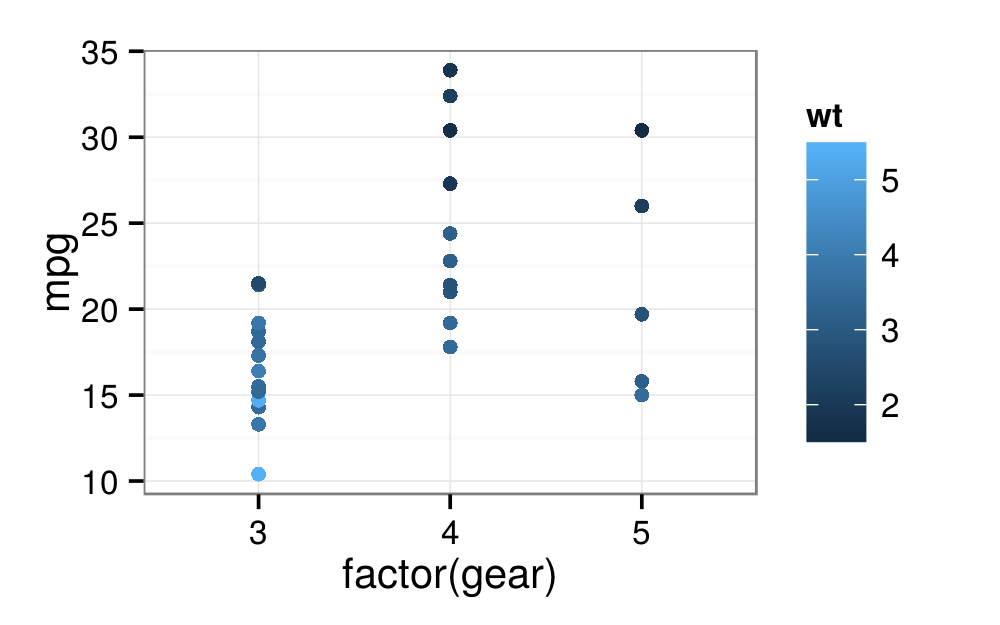
\includegraphics[width=.9\linewidth]{images/modifyScales1.png}

\end{block} \end{columns}
\end{frame}

\begin{frame}[fragile,label=sec-4-4]{Scale breaks and labels}
 \begin{columns} \column{.85\textwidth} \begin{block}{}

\begin{minted}[fontsize=\scriptsize]{r}
p7 <- p6 + geom_point(aes(color = wt)) +
  scale_x_discrete("Number of Gears",
		   breaks = c("3", "4", "5"),
		   labels = c("Three", "Four", "Five"))
p7 + scale_color_continuous("Weight",
			 breaks = with(mtcars, c(min(wt), median(wt), max(wt))),
			 labels = c("Light", "Medium", "Heavy"))
\end{minted}

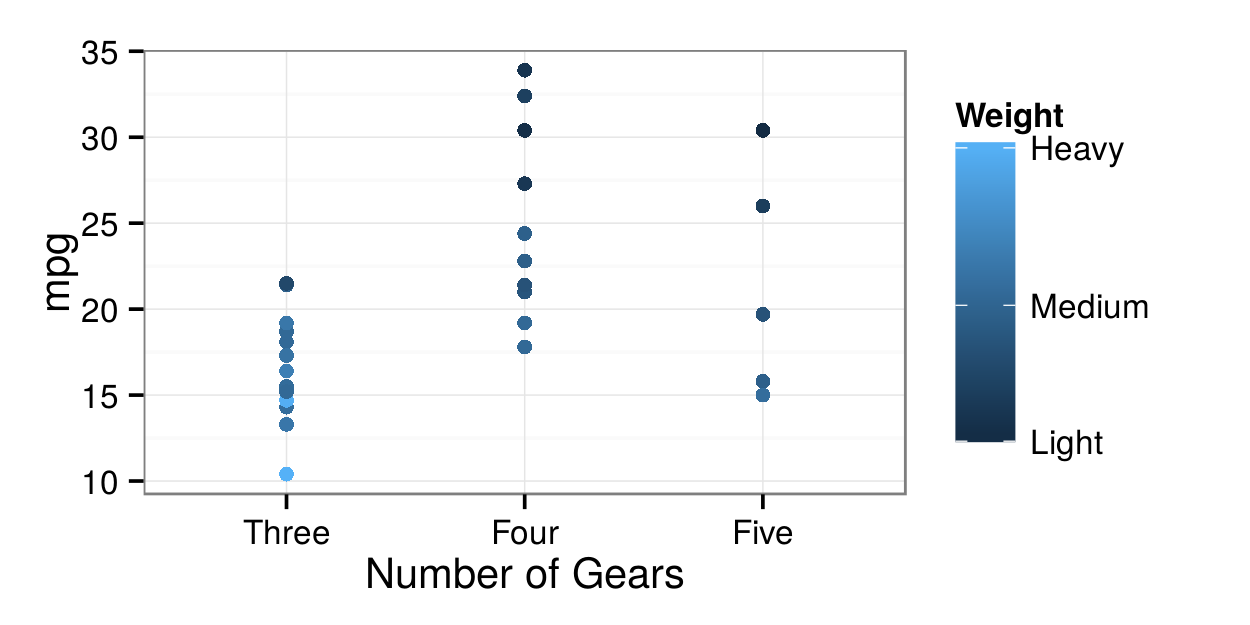
\includegraphics[width=.9\linewidth]{images/modifyScales2.png}

\end{block} \end{columns}
\end{frame}

\begin{frame}[fragile,label=sec-4-5]{Scale breaks and labels}
 \begin{columns} \column{.85\textwidth} \begin{block}{}

\begin{minted}[fontsize=\scriptsize]{r}
p7 + scale_color_continuous("Weight",
			 breaks = with(mtcars, c(min(wt), median(wt), max(wt))),
			 labels = c("Light", "Medium", "Heavy"),
			 low = "black",
			 high = "gray80")
\end{minted}

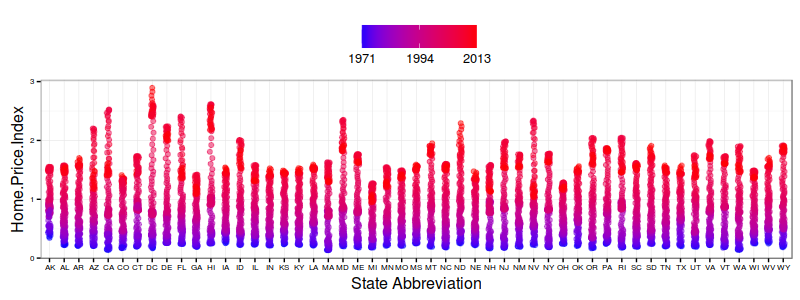
\includegraphics[width=.9\linewidth]{images/modifyScales3.png}

\end{block} \end{columns}
\end{frame}

\begin{frame}[fragile,label=sec-4-6]{Using different color scales}
 \begin{columns} \column{.85\textwidth} \begin{block}{}

\begin{minted}[fontsize=\scriptsize]{r}
p7 + scale_color_gradient2("Weight",
			  breaks = with(mtcars, c(min(wt), median(wt), max(wt))),
			  labels = c("Light", "Medium", "Heavy"),
			  low = "blue",
			  mid = "black",
			  high = "red",
			  midpoint = median(mtcars$wt))
\end{minted}

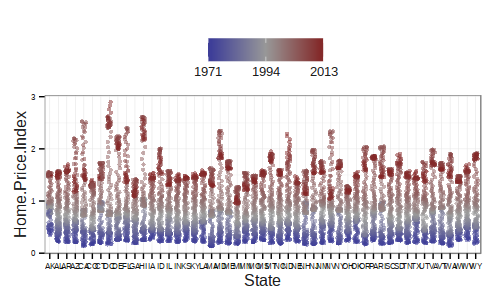
\includegraphics[width=.9\linewidth]{images/modifyScales4.png}

\end{block} \end{columns}
\end{frame}

\begin{frame}[fragile,label=sec-4-7]{Scale Modification Examples}
 \begin{columns} \column{.85\textwidth} \begin{block}{}

\begin{minted}[fontsize=\scriptsize]{r}
p8 <- ggplot(mtcars, aes(x = factor(gear), y = mpg))
p8 + geom_point(aes(size = wt))
\end{minted}

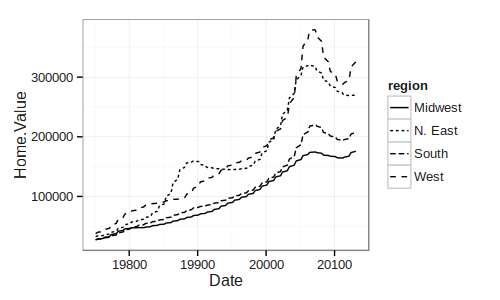
\includegraphics[width=.9\linewidth]{images/modifyScales5.png}

\end{block} \end{columns}
\end{frame}

\begin{frame}[fragile,label=sec-4-8]{Scale range}
 \begin{columns} \column{.85\textwidth} \begin{block}{}

\begin{minted}[fontsize=\scriptsize]{r}
p8 + geom_point(aes(size = wt)) +
  scale_size_continuous("Weight",
			range = c(2, 10))
\end{minted}

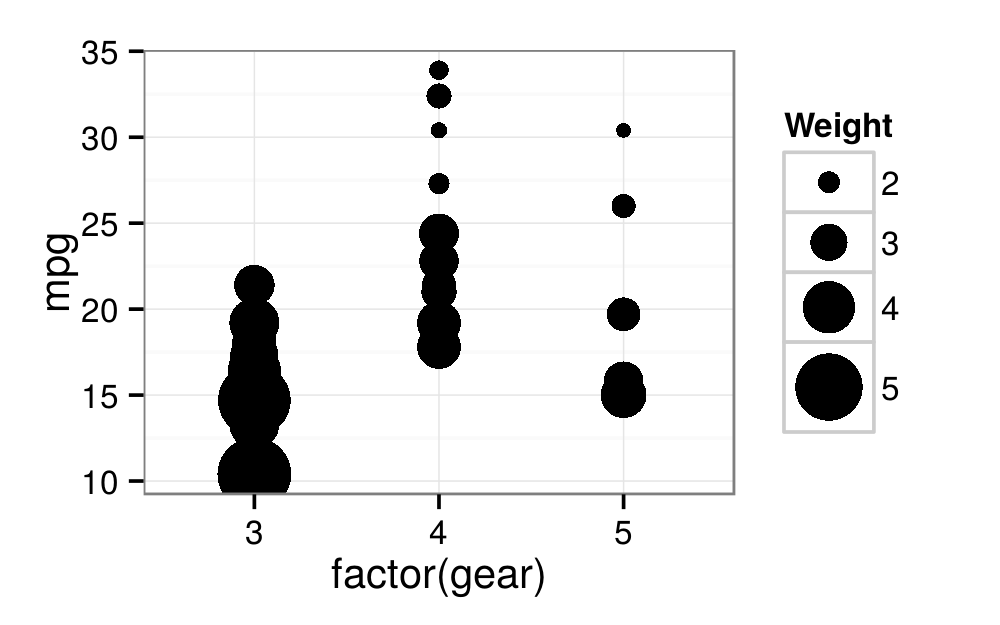
\includegraphics[width=.9\linewidth]{images/modifyScales6.png}

\end{block} \end{columns}
\end{frame}

\begin{frame}[label=sec-4-9]{Available Scales}
\begin{itemize}
\item Partial combination matrix of available scales
\end{itemize}
\begin{center}
\begin{tabular}{lll}
\alert{Scale} & \alert{Types} & \alert{Examples}\\
\hline
scale$_{\text{color}}$\_ & identity & scale$_{\text{fill}}$$_{\text{continuous}}$\\
scale$_{\text{fill}}$\_ & manual & scale$_{\text{color}}$$_{\text{discrete}}$\\
scale$_{\text{size}}$\_ & continuous & scale$_{\text{size}}$$_{\text{manual}}$\\
 & discrete & scale$_{\text{size}}$$_{\text{discrete}}$\\
 &  & \\
scale$_{\text{shape}}$\_ & discrete & scale$_{\text{shape}}$$_{\text{discrete}}$\\
scale$_{\text{linetype}}$\_ & identity & scale$_{\text{shape}}$$_{\text{manual}}$\\
 & manual & scale$_{\text{linetype}}$$_{\text{discrete}}$\\
 &  & \\
scale$_{\text{x}}$\_ & continuous & scale$_{\text{x}}$$_{\text{continuous}}$\\
scale$_{\text{y}}$\_ & discrete & scale$_{\text{y}}$$_{\text{discrete}}$\\
 & reverse & scale$_{\text{x}}$$_{\text{log}}$\\
 & log & scale$_{\text{y}}$$_{\text{reverse}}$\\
 & date & scale$_{\text{x}}$$_{\text{date}}$\\
 & datetime & scale$_{\text{y}}$$_{\text{datetime}}$\\
\end{tabular}
\end{center}
\end{frame}

\begin{frame}[label=sec-4-10]{Exercise III}
\begin{enumerate}
\item Experiment with color, size, and shape aesthetics / scales
\item What happens when you map more than one aesthetic to a variable?
\item Which aesthetics are good for continuous variables? Which work better for discrete variables?
\end{enumerate}
\end{frame}

\section{Faceting}
\label{sec-5}

\begin{frame}[fragile,label=sec-5-1]{Faceting}
 \begin{itemize}
\item Faceting is \texttt{ggplot2} parlance for \alert{small multiples}
\item The idea is to create separate graphs for subsets of data
\item \texttt{ggplot2} offers two functions for creating small multiples:
\begin{enumerate}
\item \texttt{facet\_wrap()}: define subsets as the levels of a single grouping variable
\item \texttt{facet\_grid()}: define subsets as the crossing of two grouping variables
\end{enumerate}
\item Facilitates comparison among plots, not just of geoms within a plot
\end{itemize}
\end{frame}

\begin{frame}[fragile,label=sec-5-2]{Example Data II: \texttt{Housing prices}}
 \begin{minted}[fontsize=\scriptsize]{r}
housing <- read.csv("dataSets/landdata-states.csv")
head(housing[1:5])
\end{minted}

(Data from \url{https:www.lincolninst.edu/subcenters/land-values/land-prices-by-state.asp})
\end{frame}

\begin{frame}[fragile,label=sec-5-3]{What is the trend in housing prices?}
 \begin{itemize}
\item Start by using a technique we already know--map State to color
\end{itemize}

\begin{columns} \column{.85\textwidth} \begin{block}{}

\begin{minted}[fontsize=\scriptsize]{r}
p8 <- ggplot(housing, aes(x = Date, y = Home.Value))
p8 + geom_line(aes(color = State))
\end{minted}

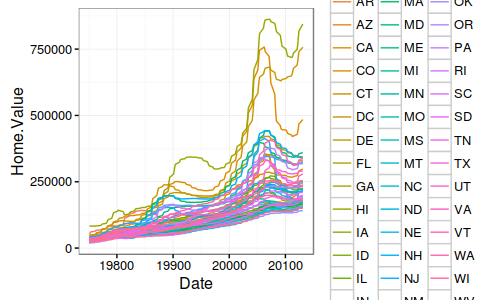
\includegraphics[width=.9\linewidth]{images/housing1.png}

\end{block} \end{columns}
\begin{itemize}
\item There are two problems here--there are too many states to distinguish each one by color, and the lines obscure one another
\end{itemize}
\end{frame}

\begin{frame}[fragile,label=sec-5-4]{Faceting to the rescue}
 \begin{itemize}
\item We can remedy the deficiencies of the previous plot by faceting by state rather than mapping state to color
\end{itemize}

\begin{columns} \column{.85\textwidth} \begin{block}{}

\begin{minted}[fontsize=\scriptsize]{r}
p8 + geom_line() +
    facet_wrap(~State, ncol = 10)
\end{minted}

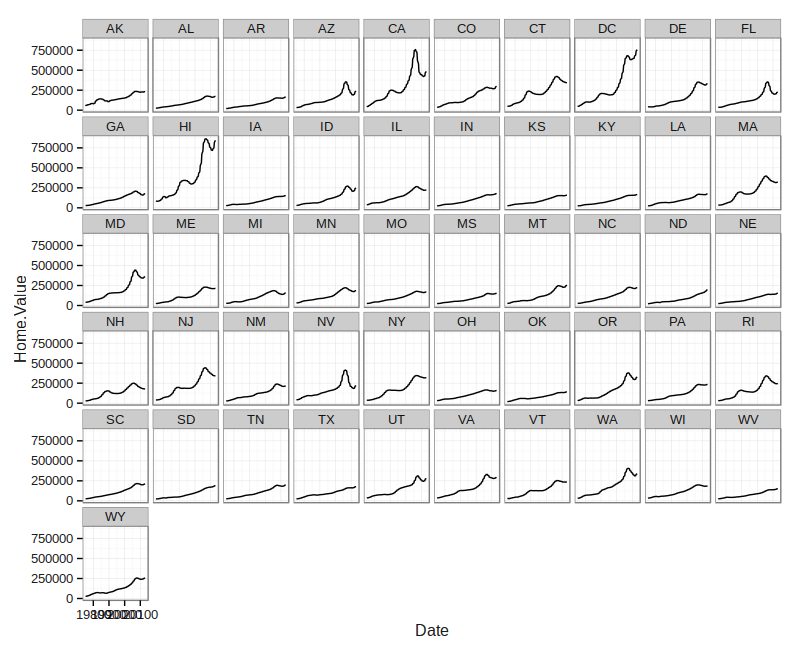
\includegraphics[width=.9\linewidth]{images/housing2.png}

\end{block} \end{columns}

\begin{itemize}
\item There is also a \verb~facet_grid()~ function for faceting in two dimensions
\end{itemize}
\end{frame}

\section{Themes}
\label{sec-6}

\begin{frame}[fragile,label=sec-6-1]{Themes}
 \begin{itemize}
\item The \verb~ggplot2~ theme system handles non-data plot elements such as
\begin{itemize}
\item Axis labels
\item Plot background
\item Facet label backround
\item Legend appearance
\end{itemize}
\item Two built-in themes:
\begin{itemize}
\item \verb~theme_gray()~ (default)
\item \verb~theme_bw()~
\item More available on the wiki:
\end{itemize}
\end{itemize}
\url{https:github.com/hadley/ggplot2/wiki/Themes}
\end{frame}

\begin{frame}[fragile,label=sec-6-2]{Overriding theme defaults}
 \begin{itemize}
\item Specific theme elements can be overridden using \verb~theme()~
\item Example:
\end{itemize}

\begin{columns} \column{.85\textwidth} \begin{block}{}

\begin{minted}[fontsize=\scriptsize]{r}
p7 + theme(plot.background = element_rect(
	    fill = "blue",
	    colour = "gray40"))
\end{minted}

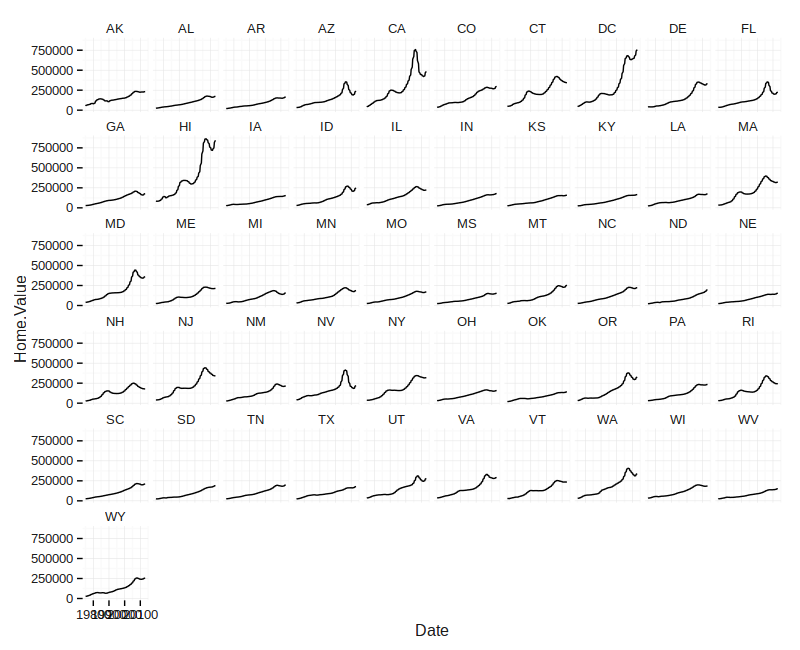
\includegraphics[width=.9\linewidth]{images/opts.png}

\end{block} \end{columns}
\begin{itemize}
\item You can see available options by printing \verb~theme_gray()~ or \verb~theme_bw()~
\end{itemize}
\end{frame}

\begin{frame}[fragile,label=sec-6-3]{Creating and saving new themes}
 \begin{itemize}
\item You can create new themes, as in the following example:
\end{itemize}

\begin{columns} \column{.85\textwidth} \begin{block}{}

\begin{minted}[fontsize=\scriptsize]{r}
theme_new <- theme_bw() +
  theme(text=element_text(size = 12, family = ""),
	axis.text.x = element_text(colour = "red"),
	panel.background = element_rect(fill = "pink"))

p7 + theme_new
\end{minted}

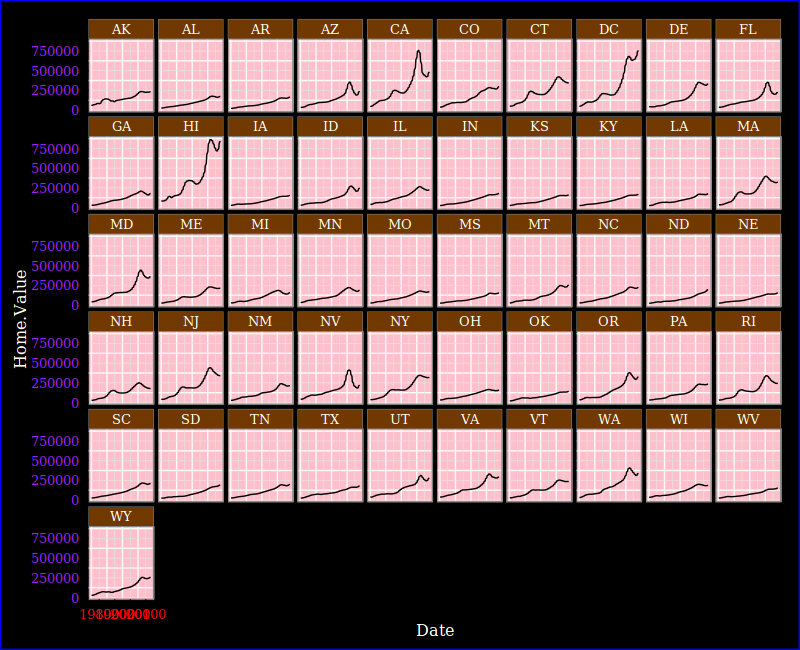
\includegraphics[width=.9\linewidth]{images/themes.png}

\end{block} \end{columns}
\end{frame}

\section{The \#1 FAQ}
\label{sec-7}
\begin{frame}[fragile,label=sec-7-1]{Map Aesthetic To Different Columns}
 The most frequently asked question goes something like this: \emph{I have two variables in my data.frame, and I'd like to plot them as separate points, with different color depending on which variable it is. How do I do that?}
\begin{columns}
\begin{column}{0.5\textwidth}

\begin{columns} \column{.85\textwidth} \begin{block}{}

\begin{minted}[fontsize=\scriptsize]{r}
ggplot(mtcars, aes(x=wt)) +
  geom_point(aes(y=disp), color="red") +
  geom_point(aes(y=hp), color="blue")


#
\end{minted}

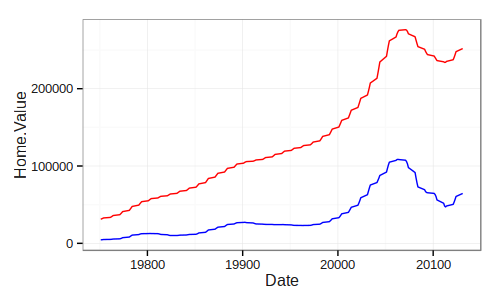
\includegraphics[width=.9\linewidth]{images/WrongWayNoMelt.png}

\end{block} \end{columns}
\end{column}

\begin{column}{0.5\textwidth}

\begin{columns} \column{.85\textwidth} \begin{block}{}

\begin{minted}[fontsize=\scriptsize]{r}
library(reshape2)
mtc.m <- melt(mtcars,
	      measure.vars=c("disp", 
			     "hp"))
ggplot(mtc.m,
       aes(x=wt,
	   y=value,
	   color=variable)) +
  geom_point()
\end{minted}

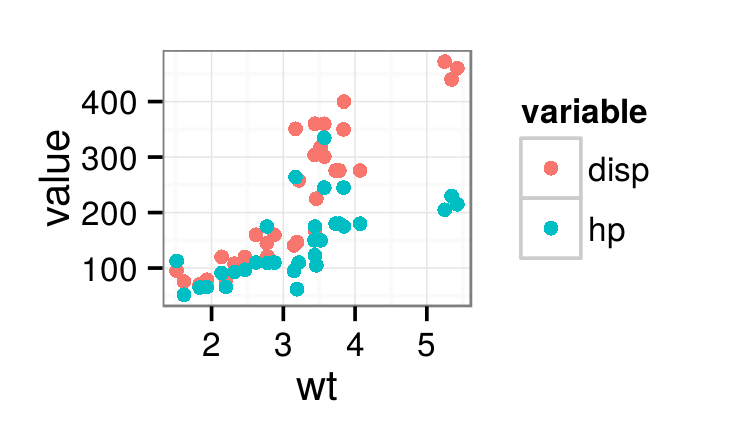
\includegraphics[width=.9\linewidth]{images/meltingDataExe.png}

\end{block} \end{columns}
\end{column}
\end{columns}
\end{frame}

\section{Putting It All Together}
\label{sec-8}

\begin{frame}[fragile,label=sec-8-1]{Challenge: Recreate This \texttt{Economist} Graph}
 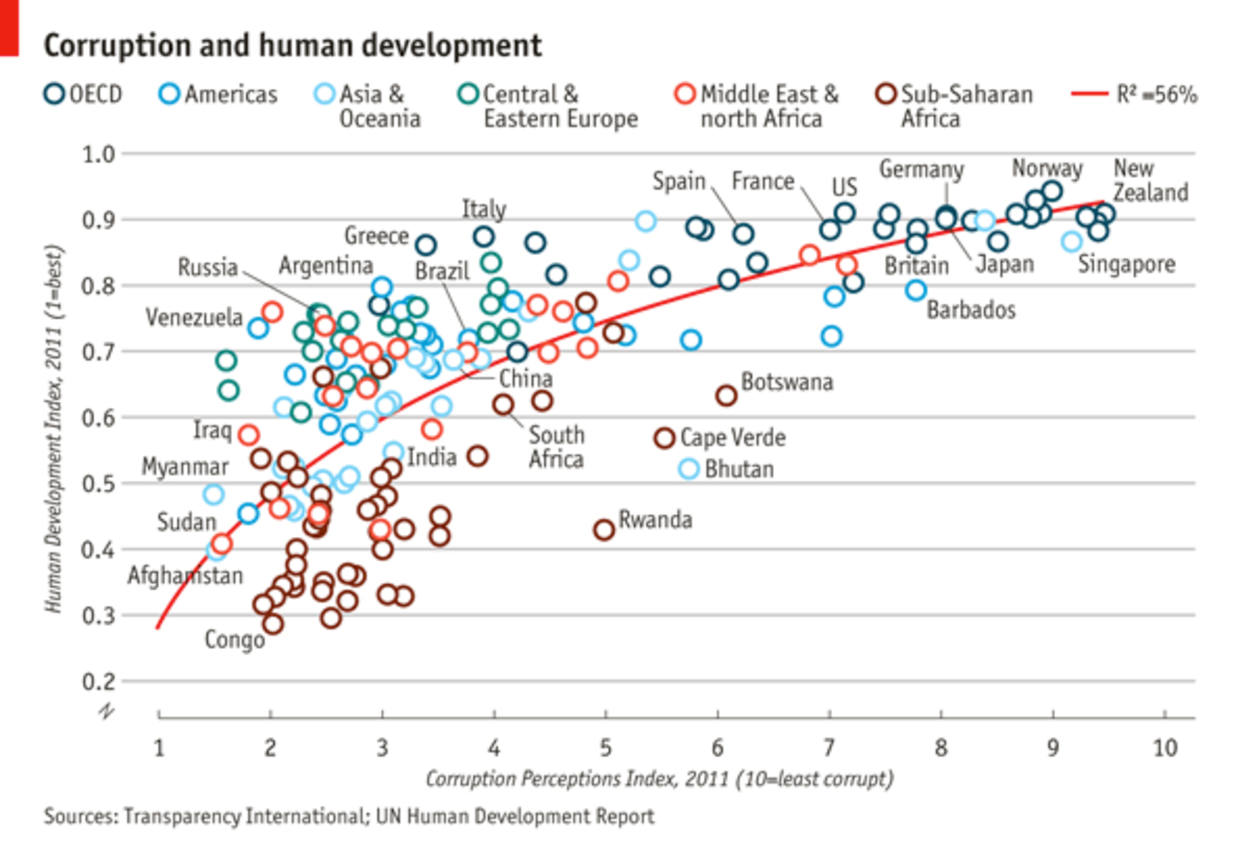
\includegraphics[width=.9\linewidth]{images/Economist1.pdf}

\small
\begin{itemize}
\item Data
\end{itemize}
The data is available in the \verb~dataSets/EconomistData.csv~ file. Read it in with \verb~dat <- read.csv("dataSets/EconomistData.csv")~
Original sources are

\tiny

\url{http:www.transparency.org/content/download/64476/1031428}
\url{http:hdrstats.undp.org/en/indicators/display_cf_xls_indicator.cfm?indicator_id=103106&lang=en}

\small
\begin{itemize}
\item Graph source:
\end{itemize}

\tiny

\url{http:www.economist.com/node/21541178}

\small
\end{frame}

\begin{frame}[fragile,label=sec-8-2]{Challenge data}
 \begin{enumerate}
\item Load the data:
\end{enumerate}
\begin{minted}[fontsize=\scriptsize]{r}
dat <- read.csv("dataSets/EconomistData.csv")
\end{minted}

\begin{enumerate}
\item Recreate this graph:
\end{enumerate}
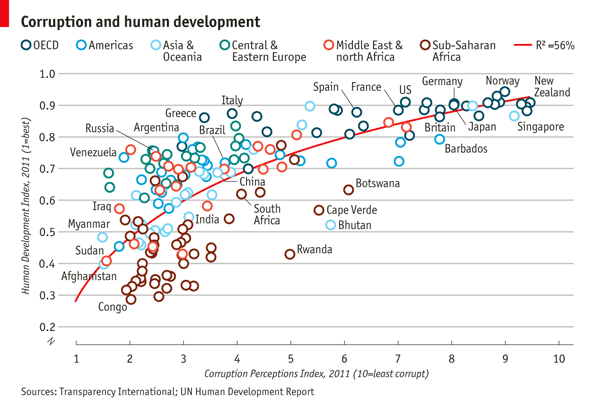
\includegraphics[width=.9\linewidth]{images/Economist1.png}
\end{frame}

\begin{frame}[fragile,label=sec-8-3]{Challenge Solution}
 Create basic scatter plot

\begin{columns} \column{.85\textwidth} \begin{block}{}

\begin{minted}[fontsize=\scriptsize]{r}
  pc1 <- ggplot(dat, aes(x = CPI, y = HDI, color = Region))
  (pc1 <- pc1 + geom_point(shape = 1))




#
\end{minted}

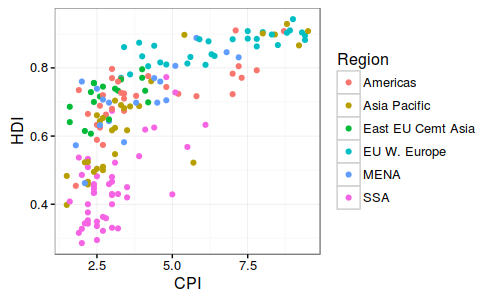
\includegraphics[width=.9\linewidth]{images/econScatter1.png}

\end{block} \end{columns}
\end{frame}

\begin{frame}[fragile,label=sec-8-4]{Challenge Solution}
 Add labels

\begin{columns} \column{.85\textwidth} \begin{block}{}

\begin{minted}[fontsize=\scriptsize]{r}
label.these <- c("Congo", "Sudan", "Afghanistan", "Greece", "China",
		 "India", "Rwanda", "Spain", "France", "United States",
		 "Japan", "Norway", "Singapore")
(pc2 <- pc1 +
 geom_text(aes(label = Country),
	   color = "black", size = 3, hjust = 1.1,
	   data = dat[dat$Country %in% label.these, ]))
\end{minted}

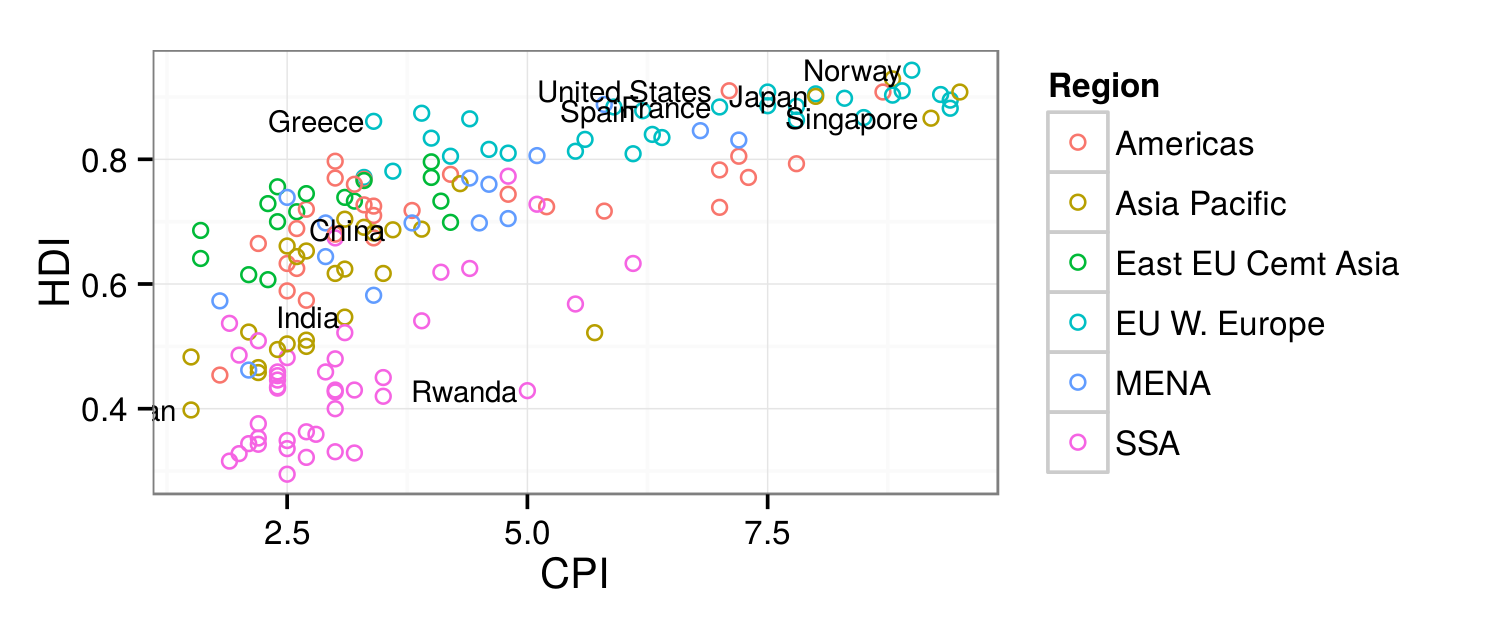
\includegraphics[width=.9\linewidth]{images/econScatter2.png}

\end{block} \end{columns}
\end{frame}

\begin{frame}[fragile,label=sec-8-5]{Challenge Solution}
 Add smoothing line

\begin{columns} \column{.85\textwidth} \begin{block}{}

\begin{minted}[fontsize=\scriptsize]{r}
  (pc3 <- pc2 +
   geom_smooth(aes(group = 1),
	       method = "lm",
	       color = "black",
	       formula = y~ poly(x, 2),
	       se = FALSE))
#
\end{minted}

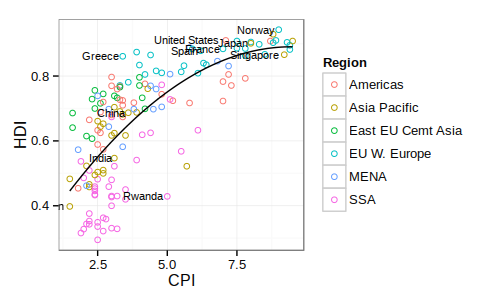
\includegraphics[width=.9\linewidth]{images/econScatter3.png}

\end{block} \end{columns}
\end{frame}

\begin{frame}[fragile,label=sec-8-6]{Challenge Solution}
 Finishing touches

\begin{columns} \column{.85\textwidth} \begin{block}{}

\begin{minted}[fontsize=\scriptsize]{r}
(pc4 <- pc3 + theme_bw() +
  scale_x_continuous("Corruption Perceptions Index, 2011\n(10 = least corrupt)") +
  scale_y_continuous("Human Development Index, 2011\n(1 = best)") +
  theme(legend.position = "top", legend.direction = "horizontal"))
\end{minted}

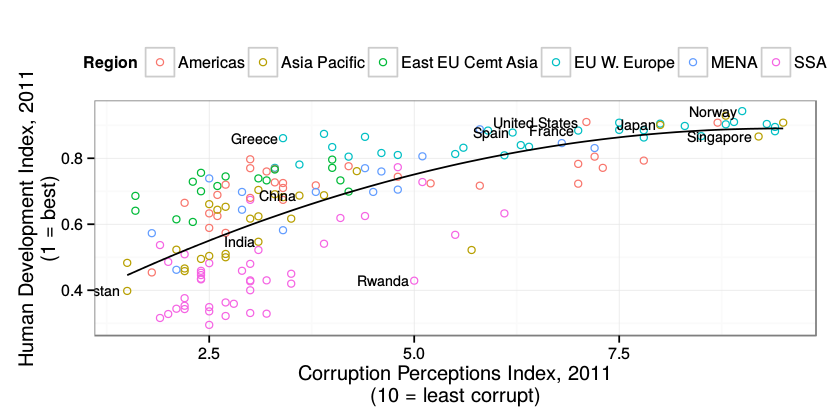
\includegraphics[width=.9\linewidth]{images/econScatter4.png}

\end{block} \end{columns}
\end{frame}

\section{Wrap-up}
\label{sec-9}

\begin{frame}[label=sec-9-1]{Help Us Make This Workshop Even Better!}
\begin{itemize}
\item Please take a moment to fill out a very short feedback form
\item These workshops exist for you -- tell us what you need!
\item \url{http:tinyurl.com/R-graphics-feedback}
\end{itemize}
\end{frame}

\begin{frame}[label=sec-9-2]{Additional resources}
\begin{itemize}
\item ggplot2 resources
\begin{itemize}
\item Mailing list: \url{http:groups.google.com/group/ggplot2}
\item Wiki: \url{https:github.com/hadley/ggplot2/wiki}
\item Website: \url{http:had.co.nz/ggplot2/}
\item StackOverflow: \url{http:stackoverflow.com/questions/tagged/ggplot}
\end{itemize}
\item IQSS resources
\begin{itemize}
\item Research technology consulting: \url{http:projects.iq.harvard.edu/rtc}
\item Workshops: \url{http:projects.iq.harvard.edu/rtc/filter_by/workshops}
\end{itemize}
\end{itemize}
\end{frame}
% Emacs 24.3.1 (Org mode 8.2.5h)
\end{document}